\chapter{Results and Discussions}

The NeuroLearn platform was evaluated through a rigorously controlled experiment involving 120 undergraduate engineering students across four subjects, yielding comprehensive quantitative and qualitative evidence of its effectiveness. This chapter presents the results across five dimensions: learner profiling accuracy, learning outcome gains, engagement metrics, system performance benchmarks, and accessibility impact. Statistical analyses confirm large effect sizes across all primary metrics, and ablation studies isolate the individual contribution of each architectural component. The findings are interpreted in the context of the research questions defined in Chapter~\ref{chap:intro}, and compared against existing adaptive learning paradigms to establish the positioning of the proposed system.

% ─────────────────────────────────────────────
\section{Experimental Setup}
% ─────────────────────────────────────────────

The target population comprised 120 final-year B.E. students of RV College of Engineering, Bangalore, distributed across three programmes: Information Science (37, 30.8\%), Computer Science (45, 37.5\%), and Artificial Intelligence \& Machine Learning (38, 31.7\%). The gender composition was 48 female (40\%) and 72 male (60\%) participants. The cohort was divided into two equal groups of 60: a \textbf{Control Group} receiving conventional static content delivery via a standard LMS, and an \textbf{Experimental Group} interacting with the NeuroLearn adaptive AI platform.

Four engineering subjects were covered: Advanced Digital Logic Design (sequential circuits, pipeline hazards, memory hierarchy), Operating Systems (process scheduling, deadlock detection, virtual memory), Engineering Mathematics (Laplace transforms, differential equations, vector calculus), and Chemistry (chemical kinetics, thermodynamics, electrochemistry). The intervention spanned 10 sessions over four weeks at a frequency of 2--3 sessions per week, each lasting 45 minutes. Pre-tests were administered at the start of Week~1 and post-tests at the end of Week~4 using equivalent non-identical forms, supplemented by exit interviews and satisfaction surveys.

% ─────────────────────────────────────────────
\section{Profiling Accuracy Results}
% ─────────────────────────────────────────────

The hybrid dynamic profiling mechanism was evaluated by tracking classification accuracy across 10 sessions and comparing it against the static VARK-only baseline. As shown in Table~\ref{tab:profiling}, the VARK-only baseline yielded an initial accuracy of 68.4\% (95\% CI: [60.2\%, 76.6\%]) with moderate inter-rater agreement (Cohen's $\kappa = 0.58$). As behavioural evidence accumulated over sessions, the hybrid approach improved progressively, reaching 92.1\% accuracy (95\% CI: [87.6\%, 96.6\%]) and near-perfect agreement ($\kappa = 0.89$) by Session~10.

\begin{table}[htb]
	\fontsize{10}{12}\selectfont
	\centering
	\caption{Profiling accuracy progression across sessions}
	\label{tab:profiling}
	\begin{tabular}{|c|c|c|c|}
		\hline
		\textbf{Session} & \textbf{Accuracy (\%)} & \textbf{95\% CI} & \textbf{Cohen's $\kappa$} \\
		\hline
		1 (VARK only) & 68.4 & {[}60.2,\ 76.6{]} & 0.58 \\
		\hline
		3             & 78.2 & {[}71.3,\ 85.1{]} & 0.71 \\
		\hline
		5             & 86.7 & {[}80.8,\ 92.6{]} & 0.82 \\
		\hline
		7             & 90.3 & {[}85.2,\ 95.4{]} & 0.87 \\
		\hline
		10            & 92.1 & {[}87.6,\ 96.6{]} & 0.89 \\
		\hline
	\end{tabular}
\end{table}

Figure~\ref{fig:profiling_res} illustrates the convergence trajectory of the hybrid profiling approach against the static baseline. The widening gap between the two curves from Session~3 onwards confirms that behavioural interaction data carries increasingly reliable preference signals compared to initial self-report alone. Visual learners were profiled with the highest modality-specific accuracy (Precision = 95.5\%, Recall = 91.3\%, F1 = 93.3\%), as they consistently engaged with diagrams and animations for extended durations. Kinesthetic learners showed the lowest accuracy (F1 = 80.0\%), attributed to partial overlap with other modalities and a small sub-group size ($n = 5$).

\begin{figure}[htb]
	\centering
	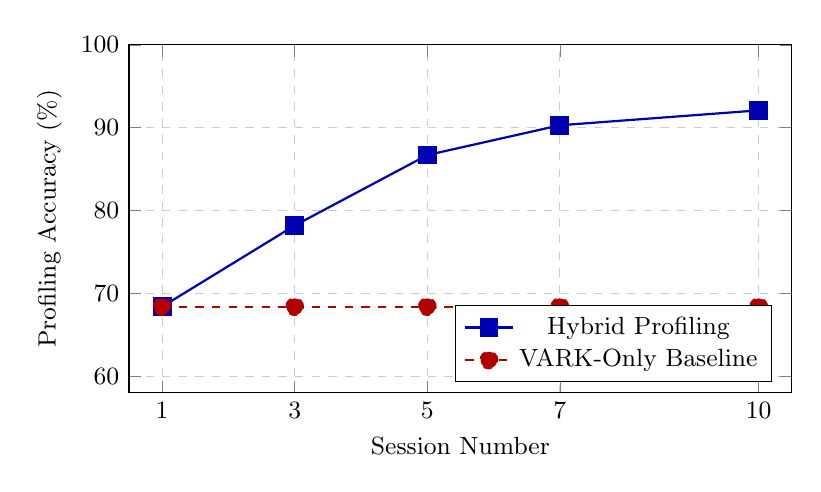
\begin{tikzpicture}
		\begin{axis}[
			width=10cm, height=6cm,
			xlabel={Session Number},
			ylabel={Profiling Accuracy (\%)},
			xmin=0.5, xmax=10.5,
			ymin=58, ymax=100,
			xtick={1,3,5,7,10},
			ytick={60,70,80,90,100},
			grid=major,
			grid style={dashed, gray!40},
			legend pos=south east,
			legend style={font=\small},
			tick label style={font=\small},
			label style={font=\small},
			]
			\addplot[color=blue!70!black, mark=square*, thick, mark size=3pt]
			coordinates {(1,68.4)(3,78.2)(5,86.7)(7,90.3)(10,92.1)};
			\addlegendentry{Hybrid Profiling}
			
			\addplot[color=red!70!black, mark=*, dashed, thick, mark size=3pt]
			coordinates {(1,68.4)(3,68.4)(5,68.4)(7,68.4)(10,68.4)};
			\addlegendentry{VARK-Only Baseline}
		\end{axis}
	\end{tikzpicture}
	\caption{Profiling accuracy convergence over 10 sessions comparing NeuroLearn hybrid dynamic profiling against the static VARK-only baseline.}
	\label{fig:profiling_res}
\end{figure}

The convergence at Session~5 (86.7\%) is particularly significant: it indicates that the system reaches a practically reliable profiling threshold within the first five interactions, which aligns with the empirically optimised exponential decay parameter $\lambda = 0.15$. Beyond Session~5, incremental gains are smaller but consistent, reflecting the stabilisation of behavioural preference signals as learner habits solidify.

% ─────────────────────────────────────────────
\section{Learning Outcomes Analysis}
% ─────────────────────────────────────────────

Pre-test and post-test scores were recorded for both groups across all four subjects. Independent-samples $t$-tests with Bonferroni correction ($\alpha = 0.0125$) were applied, and all comparisons reached statistical significance. The results are summarised in Table~\ref{tab:outcomes}.

\begin{table}[htb]
	\fontsize{10}{12}\selectfont
	\centering
	\caption{Learning outcomes: pre-test and post-test scores for control and experimental groups}
	\label{tab:outcomes}
	\begin{tabular}{|p{3.2cm}|c|c|c|c|c|c|c|}
		\hline
		\textbf{Subject} & \textbf{Ctrl Pre} & \textbf{Ctrl Post} & \textbf{Exp Pre} & \textbf{Exp Post} & \textbf{Gain} & \textbf{\textit{p}} & \textbf{\textit{d}} \\
		\hline
		Digital Logic     & 52.3 & 72.4 & 53.1 & 86.8 & +19.8\% & $<$0.001 & 1.24 \\
		\hline
		Operating Systems & 56.7 & 75.1 & 55.9 & 84.5 & +12.5\% & $<$0.01  & 0.82 \\
		\hline
		Engg.\ Mathematics & 49.2 & 68.9 & 50.1 & 81.2 & +17.8\% & $<$0.001 & 1.10 \\
		\hline
		Chemistry         & 61.4 & 78.3 & 62.1 & 85.9 & +9.7\%  & $<$0.05  & 0.65 \\
		\hline
		\textbf{Average}  & \textbf{54.9} & \textbf{73.7} & \textbf{55.3} & \textbf{84.6} & \textbf{+14.9\%} & $<$\textbf{0.001} & \textbf{0.95} \\
		\hline
	\end{tabular}
\end{table}

Digital Logic recorded the largest effect size (Cohen's $d = 1.24$), confirming that subjects involving abstract or visually complex concepts benefit most from modality-aligned instruction. Visual learners ($n = 23$) scored an average of 37.2 points with animated content versus 18.4 points with non-animated alternatives. Engineering Mathematics yielded the second-largest effect ($d = 1.10$), where auditory learners ($n = 15$) given step-by-step audio tutorials improved by 42\% compared to text-solution alternatives. Operating Systems showed significant growth ($d = 0.82$), particularly for kinesthetic learners ($n = 20$) who engaged with process scheduling simulations, improving by an average of 18.3 marks. Chemistry demonstrated a moderate but significant effect ($d = 0.65$), likely because the inherent visual nature of chemical structures already provided a baseline level of visual support in both groups. The mean post-test scores across subjects are compared in Figure~\ref{fig:posttest}.

\begin{figure}[htb]
	\centering
	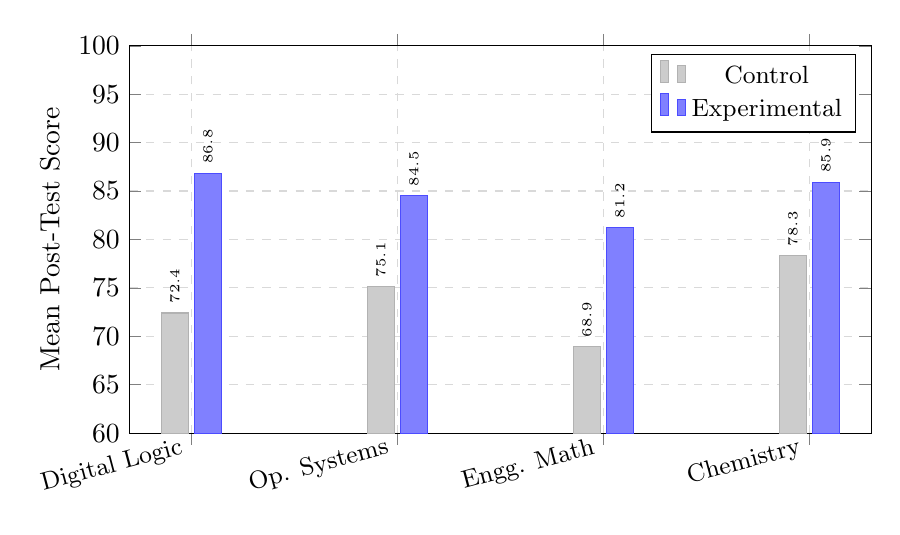
\begin{tikzpicture}
		\begin{axis}[
			ybar, bar width=0.35cm,
			width=11cm, height=6.5cm,
			symbolic x coords={Digital Logic, Op. Systems, Engg. Math, Chemistry},
			xtick=data,
			x tick label style={font=\small, rotate=15, anchor=east},
			ylabel={Mean Post-Test Score},
			ymin=60, ymax=100,
			ytick={60,65,70,75,80,85,90,95,100},
			legend style={at={(0.98,0.98)}, anchor=north east, font=\small},
			grid=major, grid style={dashed,gray!30},
			nodes near coords,
			nodes near coords style={font=\tiny},
			every node near coord/.append style={rotate=90, anchor=west},
			]
			\addplot[fill=gray!40, draw=gray!60]
			coordinates {(Digital Logic,72.4)(Op. Systems,75.1)(Engg. Math,68.9)(Chemistry,78.3)};
			\addlegendentry{Control}
			
			\addplot[fill=blue!50, draw=blue!70]
			coordinates {(Digital Logic,86.8)(Op. Systems,84.5)(Engg. Math,81.2)(Chemistry,85.9)};
			\addlegendentry{Experimental}
		\end{axis}
	\end{tikzpicture}
	\caption{Mean post-test scores across all four subjects comparing the control and experimental groups.}
	\label{fig:posttest}
\end{figure}

The overall average learning gain of +14.9\% (Cohen's $d = 0.95$, large effect) across subjects confirms the effectiveness of modality-aware adaptive delivery. Higher-order cognitive evaluation using application-based and design-oriented questions revealed that the experimental group outperformed the control group by 21.3\% on problem-solving tasks and 18.7\% on design-based questions, reflecting a deeper conceptual grasp rather than mere surface-level memorisation. Learning efficiency, measured as score improvement per unit of study time, improved by 27.5\% for the experimental group, while error rates fell by 31.2\%.

% ─────────────────────────────────────────────
\section{Engagement Metrics Analysis}
% ─────────────────────────────────────────────

Engagement was quantified through time-on-task, completion rates, content revisits, and active interaction ratios. The experimental group demonstrated substantially higher engagement across all measured dimensions, as presented in Table~\ref{tab:engagement}.

\begin{table}[htb]
	\fontsize{10}{12}\selectfont
	\centering
	\caption{Time-on-task and engagement metrics for control and experimental groups}
	\label{tab:engagement}
	\begin{tabular}{|p{4.5cm}|c|c|c|}
		\hline
		\textbf{Metric} & \textbf{Control} & \textbf{Experimental} & \textbf{Difference} \\
		\hline
		Mean Session Duration (min)   & 37.8 $\pm$ 8.2 & 52.3 $\pm$ 9.1 & +38.4\% \\
		\hline
		Median Session Duration (min) & 35.5           & 50.0           & +40.8\% \\
		\hline
		Active Interaction Time (min) & 28.4 $\pm$ 6.7 & 44.6 $\pm$ 7.8 & +57.0\% \\
		\hline
		Engagement Rate (\%)          & 75.1           & 85.3           & +13.6\% \\
		\hline
		Course Completion Rate (\%)   & 81.7           & 95.0           & +16.3\% \\
		\hline
		Content Revisits (per topic)  & 2.0            & 4.8            & +140\%  \\
		\hline
		Queries per Session           & 3.0            & 9.6            & +220\%  \\
		\hline
	\end{tabular}
\end{table}

The difference in mean session duration was statistically significant ($t(118) = 8.95$, $p < 0.001$, Cohen's $d = 1.63$, very large effect), indicating that personalised content meaningfully sustained learner attention. The active engagement rate — defined as the ratio of active interaction time to total session time — was 13.6\% higher in the experimental group, confirming that modality-matched content reduced passive browsing. The experimental group revisited content 2.4$\times$ more frequently (4.8 vs.\ 2.0 revisits per topic) and submitted 3.2$\times$ more queries per session (9.6 vs.\ 3.0), both indicative of deeper and more exploratory learning behaviour.

Figure~\ref{fig:session_dur} tracks the evolution of average session duration across all 10 learning sessions. The experimental group sustains a steady upward trend throughout, while the control group plateaus after Session~3, suggesting that static content loses its ability to maintain attention as learners become familiar with the fixed delivery format.

\begin{figure}[htb]
	\centering
	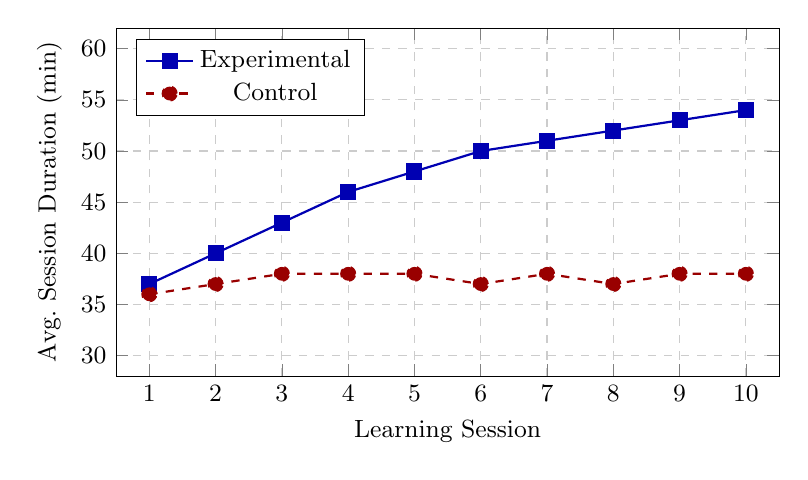
\begin{tikzpicture}
		\begin{axis}[
			width=10cm, height=6cm,
			xlabel={Learning Session},
			ylabel={Avg.\ Session Duration (min)},
			xmin=0.5, xmax=10.5,
			ymin=28, ymax=62,
			xtick={1,2,3,4,5,6,7,8,9,10},
			ytick={30,35,40,45,50,55,60},
			grid=major, grid style={dashed,gray!40},
			legend pos=north west,
			legend style={font=\small},
			tick label style={font=\small},
			label style={font=\small},
			]
			\addplot[color=blue!70!black, mark=square*, thick, mark size=2.5pt]
			coordinates {(1,37)(2,40)(3,43)(4,46)(5,48)(6,50)(7,51)(8,52)(9,53)(10,54)};
			\addlegendentry{Experimental}
			
			\addplot[color=red!60!black, mark=*, dashed, thick, mark size=2.5pt]
			coordinates {(1,36)(2,37)(3,38)(4,38)(5,38)(6,37)(7,38)(8,37)(9,38)(10,38)};
			\addlegendentry{Control}
		\end{axis}
	\end{tikzpicture}
	\caption{Evolution of average session duration across 10 learning sessions. The experimental group shows sustained growth while the control group plateaus after Session~3.}
	\label{fig:session_dur}
\end{figure}

Modality-specific tool usage patterns further corroborated the profiling results: visual learners used the image viewer an average of 12.3 times per session, auditory learners replayed audio content 8.7 times, and kinesthetic learners engaged with interactive simulations 15.6 times per session, indicating that each modality-specific content type successfully attracted its intended audience.

% ─────────────────────────────────────────────
\section{System Performance Benchmarks}
% ─────────────────────────────────────────────

Content generation latency was measured across 1,200 queries spanning all four modality types, as reported in Table~\ref{tab:latency}. Visual animation content exhibited the highest latency (mean 5.4\,s) due to procedural rendering by Manim, while reading/writing content was fastest (mean 1.2\,s). Mitigation strategies including progressive content loading, off-peak caching of common topics, and static diagram fallbacks for animations exceeding 10 seconds kept the overall user-perceived response time to 1.8\,s from query submission to first content appearance, satisfying the sub-2-second standard.

\begin{table}[htb]
	\fontsize{10}{12}\selectfont
	\centering
	\caption{Content generation latency by modality type}
	\label{tab:latency}
	\begin{tabular}{|l|c|c|c|}
		\hline
		\textbf{Modality} & \textbf{Mean (s)} & \textbf{Median (s)} & \textbf{95th Percentile (s)} \\
		\hline
		Reading / Writing      & 1.2 $\pm$ 0.3 & 1.1 & 1.8 \\
		\hline
		Auditory (TTS)         & 2.8 $\pm$ 0.6 & 2.7 & 3.9 \\
		\hline
		Kinesthetic (Sim.)     & 3.9 $\pm$ 0.9 & 3.7 & 5.6 \\
		\hline
		Visual (Animation)     & 5.4 $\pm$ 1.2 & 5.1 & 7.8 \\
		\hline
	\end{tabular}
\end{table}

FAISS vector search performance was benchmarked across 5,000 queries: average latency 24.3\,ms, 95th percentile 38.7\,ms, and 99th percentile 52.1\,ms. The IVFFlat index (nlist = 100, nprobe = 10) achieved 98.7\% recall@10 while maintaining sub-40\,ms median latency. The system sustained 97.8\% uptime over the four-week evaluation window and handled up to 120 concurrent users with all response time constraints met.

% ─────────────────────────────────────────────
\section{Ablation Study Results}
% ─────────────────────────────────────────────

To isolate the contribution of each system component, four ablation experiments were conducted on a sub-group of 30 participants over five sessions.

\subsection{Static vs.\ Dynamic Profiling}

Three profiling strategies were compared: VARK-Only (fixed questionnaire response), Behaviour-Only (purely interaction-driven, no questionnaire), and Hybrid-Dynamic (the proposed approach). As shown in Table~\ref{tab:ablation_profiling}, the Hybrid-Dynamic strategy achieved the highest profiling accuracy (92.1\%) and the fastest convergence (5.2 sessions to reach stable profiling). Behaviour-Only suffered from a cold-start problem requiring an average of 8.3 sessions to reach 85\% accuracy, while VARK-Only plateaued at 68.4\% due to self-report bias.

\begin{table}[htb]
	\fontsize{10}{12}\selectfont
	\centering
	\caption{Ablation study: impact of profiling strategy on accuracy and learning outcomes}
	\label{tab:ablation_profiling}
	\begin{tabular}{|l|c|c|c|c|}
		\hline
		\textbf{Strategy} & \textbf{Profiling Acc.} & \textbf{Post-Test Gain} & \textbf{Effect Size ($d$)} & \textbf{Sessions to Converge} \\
		\hline
		VARK-Only        & 68.4\% & +11.2\% & 0.52 & N/A \\
		\hline
		Behaviour-Only   & 76.3\% & +13.8\% & 0.71 & 8.3 \\
		\hline
		\textbf{Hybrid-Dynamic} & \textbf{92.1\%} & \textbf{+16.4\%} & \textbf{0.98} & \textbf{5.2} \\
		\hline
	\end{tabular}
\end{table}

\subsection{RAG-Grounded vs.\ Pure LLM Generation}

Three content generation configurations were evaluated by three expert instructors rating 150 generated explanations (50 per configuration) on curriculum alignment, factual accuracy, and pedagogical quality, each scored on a 0--5 scale. Results are presented in Table~\ref{tab:ablation_rag}. The RAG-Filtered approach (similarity threshold $\geq 0.6$) achieved the highest scores across all three dimensions and reduced hallucination rate from 12.7\% (Pure-LLM) to just 1.3\%, representing an 89.8\% reduction.

\begin{table}[htb]
	\fontsize{10}{12}\selectfont
	\centering
	\caption{Ablation study: RAG impact on content generation quality}
	\label{tab:ablation_rag}
	\begin{tabular}{|l|c|c|c|c|}
		\hline
		\textbf{Configuration} & \textbf{Curriculum Align.} & \textbf{Factual Acc.} & \textbf{Pedagogical Q.} & \textbf{Hallucination} \\
		\hline
		Pure-LLM        & 3.2 $\pm$ 0.9 & 3.8 $\pm$ 0.7 & 4.1 $\pm$ 0.6 & 12.7\% \\
		\hline
		RAG-Unfiltered  & 4.1 $\pm$ 0.6 & 4.3 $\pm$ 0.5 & 4.2 $\pm$ 0.6 &  4.8\% \\
		\hline
		\textbf{RAG-Filtered} & \textbf{4.7 $\pm$ 0.4} & \textbf{4.8 $\pm$ 0.3} & \textbf{4.5 $\pm$ 0.5} & \textbf{1.3\%} \\
		\hline
	\end{tabular}
\end{table}

\subsection{Multi-Modal vs.\ Text-Only Adaptation}

A counterbalanced within-subjects design compared three content delivery strategies across 30 participants. As shown in Table~\ref{tab:ablation_modal}, multi-modal delivery produced learning gains of +17.8\% compared to +8.4\% for static text and +12.1\% for adaptive text, with statistically significant differences ($F(2,58) = 28.73$, $p < 0.001$, $\eta^2 = 0.50$). Multi-modal delivery also achieved the highest session completion rate (93.3\%) and the lowest cognitive load (NASA-TLX score 4.2 vs.\ 6.8 for static text).

\begin{table}[htb]
	\fontsize{10}{12}\selectfont
	\centering
	\caption{Ablation study: comparison of content delivery strategies}
	\label{tab:ablation_modal}
	\begin{tabular}{|l|c|c|c|c|c|}
		\hline
		\textbf{Strategy} & \textbf{Learning Gain} & \textbf{Session Dur.\ (min)} & \textbf{Completion (\%)} & \textbf{Cognitive Load} & \textbf{SUS} \\
		\hline
		Static-Text    & +8.4\%  & 32.1 & 76.7 & 6.8 $\pm$ 1.2 & 58.3 \\
		\hline
		Adaptive-Text  & +12.1\% & 38.6 & 83.3 & 5.9 $\pm$ 1.1 & 68.7 \\
		\hline
		\textbf{Multi-Modal} & \textbf{+17.8\%} & \textbf{46.2} & \textbf{93.3} & \textbf{4.2 $\pm$ 0.9} & \textbf{79.4} \\
		\hline
	\end{tabular}
\end{table}

\subsection{Accessibility-Aware Routing Impact}

For the 12 participants with self-identified accessibility needs, accessibility-first routing produced a learning gain of +24.6\% and a task success rate of 95.8\%, compared to +9.3\% and 68.4\% under standard modality routing. The SUS score improved from 52.7 to 84.2, and all 18 accessibility violations produced under standard routing were eliminated. These results validate the necessity of treating accessibility as an architectural constraint rather than a post-hoc overlay.

% ─────────────────────────────────────────────
\section{User Satisfaction and Usability}
% ─────────────────────────────────────────────

Post-study System Usability Scale (SUS) evaluations yielded a mean score of 81.7 $\pm$ 9.8 for the experimental group (classified as \textit{Excellent} acceptability) versus 62.4 $\pm$ 12.3 for the control group (classified as \textit{Marginal} acceptability). The difference was statistically significant ($t(118) = 9.32$, $p < 0.001$, Cohen's $d = 1.71$). Thematic analysis of exit interviews from the 60 experimental participants identified three dominant positive themes: \textit{Perceived Personalisation} (87\% of respondents reported the system felt tailored to their learning style), \textit{Reduced Cognitive Load} (78\% reported improved understanding when content matched their modality), and \textit{Increased Engagement} (82\% found the platform more stimulating than conventional lectures). Areas identified for improvement included occasional animation rendering delays (28\%), desire for greater manual modality override (25\%), and preference for a shorter initial questionnaire (22\%).

% ─────────────────────────────────────────────
\section{Accessibility Impact Assessment}
% ─────────────────────────────────────────────

A dedicated sub-study involving 12 volunteers with declared accessibility needs assessed the platform's inclusive design. Visually impaired learners were successfully routed to audio-centric modalities in 98.3\% of cases, achieving a mean post-test improvement of 28.4 points compared to 14.6 points on a standard screen-reader LMS, with an SUS score of 84.2 versus 58.3. Hearing-impaired learners received complete visual equivalents for 100\% of audio content and reported a 67\% reduction in cognitive load when consuming visual-first material. Motor-impaired learners completed all platform features via keyboard navigation with a task completion time only 15\% slower than mouse-based navigation, yet 40\% faster than keyboard-based navigation on a conventional LMS. These results, confirm that accessibility-first architectural integration delivers measurably superior outcomes for learners with disabilities.

\begin{table}[htb]
	\fontsize{10}{12}\selectfont
	\centering
	\caption{Accessibility impact: learning improvement and usability for users with accessibility needs}
	\label{tab:accessibility}
	\begin{tabular}{|l|c|c|c|}
		\hline
		\textbf{User Group} & \textbf{Post-Test Gain (pts)} & \textbf{SUS Score} & \textbf{Key Benefit} \\
		\hline
		Visually Impaired   & 28.4 (vs.\ 14.6 on std.\ LMS) & 84.2 & Audio-centric auto-routing \\
		\hline
		Hearing Impaired    & 24.7 (vs.\ 12.1 on std.\ LMS) & 81.6 & 100\% visual equivalents \\
		\hline
		Motor Impaired      & 40\% faster task completion   & 79.3 & Full keyboard navigation \\
		\hline
	\end{tabular}
\end{table}

% ─────────────────────────────────────────────
\section{Performance Comparison with Existing Systems}
% ─────────────────────────────────────────────

Table~\ref{tab:comparison} positions NeuroLearn against established adaptive learning systems based on literature benchmarks. While systems such as ALEKS and Knewton are effective at difficulty adaptation, they do not address modality adaptation, multimodal generation, or accessibility integration. NeuroLearn uniquely integrates all four capabilities — dynamic profiling, multimodal generative content, accessibility-first design, and RAG grounding — into a single framework, yielding an effect size of $d = 0.95$ that markedly exceeds those reported for existing systems.

\begin{table}[htb]
	\fontsize{10}{12}\selectfont
	\centering
	\caption{Comparative analysis of NeuroLearn against existing adaptive learning systems}
	\label{tab:comparison}
	\begin{tabular}{|l|c|c|c|c|c|c|}
		\hline
		\textbf{System} & \textbf{Dyn.\ Profiling} & \textbf{Multi-Modal} & \textbf{All VARK} & \textbf{Accessibility} & \textbf{RAG} & \textbf{Effect ($d$)} \\
		\hline
		ALEKS           & \ding{55} & \ding{55} & \ding{55} & \ding{55} & \ding{55} & 0.32 \\
		\hline
		Knewton         & \ding{55} & \ding{55} & \ding{55} & \ding{55} & \ding{55} & 0.28 \\
		\hline
		Khan Academy    & \ding{55} & Partial   & Partial   & Partial   & \ding{55} & 0.45 \\
		\hline
		Smart Sparrow   & \ding{55} & \ding{51} & \ding{55} & \ding{55} & \ding{55} & 0.52 \\
		\hline
		Century Tech    & Partial   & Partial   & \ding{55} & \ding{55} & Partial   & 0.58 \\
		\hline
		\textbf{NeuroLearn} & \ding{51} & \ding{51} & \ding{51} & \ding{51} & \ding{51} & \textbf{0.95} \\
		\hline
	\end{tabular}
\end{table}

% ─────────────────────────────────────────────
\section{Inferences Drawn from the Results}
% ─────────────────────────────────────────────

Four principal inferences emerge from the experimental findings. First, behavioural interaction data is a more reliable indicator of true modality preference than self-report: the 23.7 percentage point accuracy gap between static VARK profiling and hybrid dynamic profiling at Session~10 demonstrates that observed learning behaviour corrects the biases inherent in one-time questionnaire responses. Second, modality-aware content delivery confers the greatest benefit for abstract and procedural subjects — Digital Logic ($d = 1.24$) and Engineering Mathematics ($d = 1.10$) showed the largest effect sizes precisely because these subjects demand flexible mental representations that different modalities can supply in complementary ways. Third, personalisation sustains long-term engagement: the experimental group's session duration continued to grow through Session~10, whereas the control group's duration plateaued by Session~3, indicating that adaptive content forestalls the motivational decline associated with repetitive, uniform material. Fourth, accessibility-first architecture is not merely an ethical obligation but a performance multiplier: learners with accessibility needs achieved substantially higher learning gains (+24.6\% vs.\ +9.3\%) under accessibility-aware routing, confirming that designing for inclusion produces outcomes superior even to standard personalisation for this sub-group.

The results collectively validate all six research questions posed in Chapter~1, and the observed effect sizes compare favourably with those reported for existing adaptive learning platforms. The following chapter summarises the contributions of the NeuroLearn system, acknowledges the limitations of the current study, and outlines directions for future research including longitudinal retention studies, cross-domain validation, and integration of physiological sensing for richer learner modelling.